%\documentclass[12pt, a4paper]{scrartcl}
%\usepackage[german]{babel}
%\usepackage[utf8]{inputenc}
%\usepackage{graphicx}
%
%\usepackage{listings}
%
%\begin{document}
\section{Funktionsumfang und Eingabeverarbeitung auf der Anwendungsebene}

\subsection{Entwicklung einer eigenen Scriptsprache zur Anwendungssteuerung}
\subsubsection{Theoretische Grundlagen formaler Sprachen}
Wir als Menschen haben die gesprochenen Sprachen entwickelt, um uns untereinander zu verständigen und Informationen auszutauschen. 
Um Missverständnisse zu vermeiden, ist unsere Kommunikation durch strikte grammatikalische und semantische Regeln definiert. 
Es werden strukturelle Merkmale, wie zum Beispiel die Reihenfolge einzelner Sprachteile festgelegt, außerdem gibt es einen begrenzten Wortschatz, in dem jedes Wort eine bestimmte Bedeutung hat.
Um auch Computern Informationen zu übermitteln, und eine maschinelle Verarbeitung dieser zu ermöglichen, benutzt man formale Sprachen. 
Diese gleichen von den grundlegenden strukturellen Ansprüchen den natürlichen Sprachen, verfügen also auch über eine Syntax und eine Semantik, definieren sich allerdings dadurch, dass diese für einen Rechner eindeutig verständlich sein müssen, und demnach kein Interpretationsfreiraum gelassen wird. Ziel ist es klare Anweisungen in einer für den Computer verständlichen Weise zu übermitteln.\\\\
Da Sprachen in der Regel durch das Aneinanderreihen von einzelnen Sprachelementen über eine Unendlichkeit verfügen, nutzt man künstliche Grammatiken der Form $G = (N, T, P, s)$, um diese zu beschreiben. 
Eine Grammatik $G$ dieser Art verfügt über eine Menge von nichtterminalen Symbolen $N$, auch Variablen genannt, welche im Verlauf der Wortbildung durch die Menge der Produktionsregeln $P$ der Form $U \rightarrow V$ durch eine Kombination aus terminalen Zeichen der Menge $T$ ersetzt werden. 
Das Startsymbol $s$ ist zwingend die erste Variable, welche durch eine Produktion der Form $s \rightarrow V$ ersetzt wird. 
Ein Wort gehört einer Grammatik $G$ an, wenn es nur noch aus terminalen Symbolen der Menge $T_G$ besteht und ausgehend von dem Startsymbol $S_G$ mit den Produktionen der Menge $P_G$ gebildet werden kann.\footnote{$	https://www.uni-ulm.de/fileadmin/website\_uni\_ulm/iui.inst.040/Formale\_Methoden\_der\_Informatik$\\$/Vorlesungsskripte/FMdI-06--2010-01-10--FormaleSprachen\_Vorlesung.pdf$
; 19.11.2018}\\\\
Je nachdem, wie die Produktionsregeln einer Grammatik aufgebaut sind, lässt sich eine formale Sprache nach dem Informatiker Noam Chomsky in vier Typen einteilen. 
Grundsätzlich gehört jede Sprache dem Typ 0 der allgemeinen Sprachen an. 
Eine Sprache gehört immer einem Typ $X$ an, wenn alle Bedingungen  der Typen $\leq X$ für alle Produktionsregeln der Form $U \rightarrow V$ erfüllt sind. 
Die Bedingung für eine kontextsensitive Sprache des Typs 1 besagt, dass durch eine Produktionsregel das Wort nicht verkürzt werden kann, also $|U| \leq |V|$. 
Für eine kontextfreie Sprache des Typs 2 gilt, dass durch eine Produktionsregel nur jeweils eine Variable ersetzt werden kann, also $|U| = 1$. 
Eine Sprache ist eine reguläre Sprache des Typs 3, wenn ein nichtterminales Symbol mit einer Produktionsregel durch ein terminales Symbol und ein optionales nichtterminales Symbol ersetzt wird, jedoch nicht durch mehre, also $U \leq a|aB$. \footnote{I. Wegener;	Theoretische Informatik; Kap.5}\\
\begin{table}[h!]
\centering
\begin{tabular}{|ll|ll|}
\hline
Verwendung                    & Zeichen   & Verwendung                    & Zeichen \\ \hline
Definition                    & =         & Aufzählung                    & ,       \\
Endezeichen                   & ;         & Alternative                   & |       \\
Option                        & {[}...{]} & Optionale Wiederholung        & \{...\} \\
Gruppierung                   & (....)    & Anführungszeichen 1. Variante & "..."   \\
Anführungszeichen 2. Variante & '...'     & Kommentar                      & (*...*) \\
Spezielle Sequenz             & ?...?     & Ausnahme                      & -       \\ \hline
\end{tabular}
\caption{Inhalt der Erweiterten-Backus-Nauer-Form}
\label{ebnf}
\end{table}
Um die Darstellung von Sprachen zu vereinheitlichen, wurde die Erweiterte-Backus-Nauer-Form, kurz EBNF entwickelt. 
Die oben gegebenen Zeichen sind Teil des EBNF ISO-Standards und durch sie lässt sich jede beliebige formale Sprache beschreiben.\\
 
\subsubsection{Spezifikation unserer Skriptsprache anhand unserer Ansprüche an den Funktionsumfang}
Für unser Programm haben wir uns grundlegend vorgenommen Funktionen für das Versenden von Dateien sowie Befehlen an einen zweiten PC bereitzustellen. 
Es erfordert also in gewissem Maße eine Kommunikation zwischen dem Nutzer und dem Programm, um die Wünsche des Bedieners genauer zu spezifizieren und der Software zu übermitteln. 
Um dies zu bewerkstelligen entschieden wir uns, eine eigene formale Sprache zu entwickeln, mit dem Ziel Befehle an das Programm mit den entsprechenden Argumenten zu übermitteln, welche über ein Konsolenfenster eingegeben werden.
Unsere Sprache sollte Folgende Anweisungen beinhalten:\\
\begin{table}[h!]
\centering
\begin{tabular}{|ll|}
\hline
Befehl & Argumente \\ \hline
send\_file & file\_name \\
send\_comm & return command\_name {[}arguments{]} \\
get\_file & file\_name \\
connect & ip\_address \\
disconnect & \\
reconnect & ip\_address \\
shutdown [send\_comm] & \\
open [send\_file] & file\_name \\
chat & chat\_msg \\
squit & \\ \hline
\end{tabular}
\caption{Befehlssatz der Eingabesyntax}
\label{befehl}
\end{table}\\
Die Befehle $send\_file$ und $send\_comm$ sind hierbei die allgemeinen Funktionen zum Senden einer Datei oder eines Befehls an die betriebssystemeigene Kommandozeile jeglicher Art. Das Kommando $get\_file$ ist identisch zu $send\_file$ mit dem Unterschied, dass eine Datei von dem angefragten PC auf den anfragenden übertragen werden soll. Mit den Anweisungen ($dis-$/$re-$)$connect$ wird der grundlegende Verbindungsaufbau gesteuert. Durch den $connect$-Befehl wird versucht eine Verbindung zu der als Argument übergebenen IP-Adresse zu errichten. $disconnect$ bewirkt die Beendigung einer bestehenden Verbindung, $reconnect$ versucht zusätzlich eine neue Verbindung zu erstellen. 
$shutdown$ und $open$ sind spezielle versendete Anweisungen zum Herunterfahren des Zielcomputers und Öffnen einer Datei, bei denen wir es aufgrund ihrer frequentierten Nutzung für sinnvoll hielten sie eigenständig in unsere formale Sprache zu integrieren. Sie basieren auf den zwei Grundfunktionen und stehen beispielhaft für die Erweiterbarkeit des Funktionsumfangs unserer Software. Durch den $chat$ Befehl lässt sich eine Textnachricht an den Verbundenen Rechner senden.
Zusätzlich für Befehle, welche mit Dateien arbeiten sollen, muss der Dateiname beziehungsweise der Dateipfad als Zeichenkette angefügt werden. 
Die Übermittlungsfunktionen für Anweisungen benötigen neben dem Anweisungsnamen als Zeichenkette auch optionale Argumente, mit welchen die Anweisung in der Kommandozeile ausgeführt werden soll. Außerdem wird der Flag $return$ benötogt, welcher bestimmt, ob das Ergebnis des Übertragenen Befehls zurück an den Ausgangscomputer gesenet werden soll. Zum beenden des Programms existiert die Anweisung $squit$, sie implementiert eine Alternative zu den grafischen Möglichkeiten zum beende\\\\
Um unsere formale Sprache zu implementieren entwickelten wir zuerst als Grundlage eine Darstellung der Eweiterten-Backus-Nauer-Form. Eine solche Darstellung hat den Vorteil einer unkomplizierten Übertragung der Produktionsregeln in die Implementierung, welche die Nutzereingaben überprüft. Im späteren Verlauf der Entwicklung wurden einzelne Befehle und Argumente angefügt und verändert, um eine Praxistauglichkeit zu bewirken.

\subsection{Implementierung der Anwendungssteuerung in der Skriptsprache Lua}

\subsubsection{Darstellung des grundlegenden Programmaufbaus und Programmablaufs}
Grundlegende Aufgabe der Anwendungssteuerung ist es die Eingaben, die der Nutzer unserer Software tätigt, in Aktionen des Programms umzusetzen. 
Dazu wird zum einen auf dem Startrechner die nach der in Kapitel 1.1 beschriebenen Syntax eingegebene Anweisung in der Eingabeverarbeitung auf ihre Korrektheit überprüft um anschließend aufgeschlüsselt zu werden und die gewünschte Sendefunktion zu initialisieren.\\
Nachdem die Daten mithilfe des Netzwerkprotokolls übermittelt wurden, werden sie von der Übertragungsverarbeitung auf dem Empfängercomputer weiter bearbeitet. Je nach spezifiziertem Typ der Übermittlung wird entweder die enthaltene Datei auf Fehler überprüft und anschließend endgültig gespeichert, oder die auszuführende Anweisung wird an die betriebsystemeigene Kommandozeile weitergegeben und ausgeführt.\\
Um keine ungewollten Übertragungen von potenziell schädlichen Dateien oder Anweisungen zu ermöglichen wird für die Ausführung jeder Übermittlungsanfrage die Bestätigung des Empfängers benötigt, sofern nicht der $root-Modus$ aktiviert ist. Als $root$-Nutzer hat man uneingeschränkte Kontrolle über den Ziel-Computer, was besonders für administrative Tätigkeiten sinnvoll ist.\\\hfill\\ 
\begin{figure}[h!]
\centering
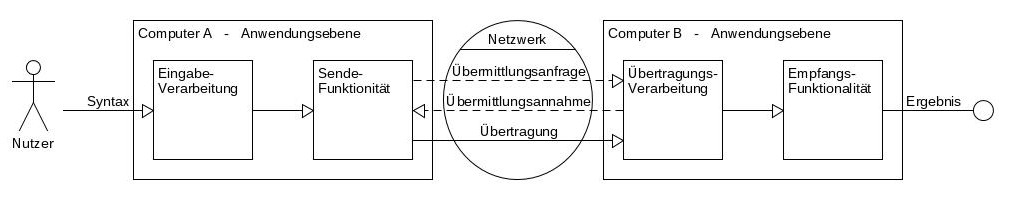
\includegraphics[scale=.45]{anw.jpg}
\label{anw}
\caption{Schematische Darstellung der Ablaufenden Prozesse im Programm}
\end{figure}

\subsubsection{Ansprüche an die Implementierung und die daraus resultierende Wahl der Programmiersprache}
Wie in Kapitel 1.2.1 erläutert, wird auf der Anwendungsebene unseres Programmes, also dem Teil, welcher nicht für die Kommunikation im Netzwerk zuständig ist, die grundlegende Funktionalität implementiert. Da unser selbstentwickeltes Netzwerkprotokoll, welches die eigentliche Kommunikation zwischen 2 Computern regelt, relativ universell auf verschiedenartige Daten anwendbar ist, stellt dieses im Bezug auf den Funktionsumfang der Software nicht den limitierenden Faktor da. Um das Protokoll eventuell auch im Zeitraum nach der eigentlichen Arbeit ausnutzen zu können, und nicht durch einen festgelegten Satz von Befehlen beschränkt zu werden, entschieden wir uns dazu diesen Programmteil in einer Skriptsprache zu implementieren.
Diese Klasse von Programmiersprachen zeichnet sich dadurch aus, dass der vom Menschen lesbare Quelltext eines Programmes erst bei seiner Ausführung in Anweisungen übersetzt wird, welche für den Computer ausführbar sind. Im Gegensatz zu kompilierten Sprachen hat dies den Vorteil, dass der Programmcode unkompliziert korrigiert und modifiziert werden kann und sofort lauffähig ist.\\\\
In diesem Zusammenhang ergibt sich außerdem eine leichte Wartbarkeit, also die Möglichkeit eventuell auftretende Fehler zu beseitigen, als ein weiterer erfüllter Anspruch.\\
Den Vorteil von kompilierten Programmiersprachen, dass sie sich durch eine höhere Leistungsfähigkeit besonders bei komplexeren Problemen auszeichnen, haben wir uns durch die Implementierung unseres Netzwerkteils in der Sprache C++ zu Nutz gemacht. Dies stellt den Anspruch, dass die gewählte Skriptsprache problemlos in Software der Sprache C++ einzubetten ist, und keine Probleme an der Schnittstelle der beiden Programmteile mit zwei unterschiedlichen Sprachen auftreten.\\\\
Da wir als Gruppenmitglieder unterschiedliche Betriebsysteme auf unseren Arbeitsrechnern benutzen, entstand als Nebenprodukt die Anforderung, dass das finale Programm systemunabhängig sein muss, also ohne erheblichen Aufwand auf neue Betriebssysteme portierbar ist. 
Unser Fokus lag dabei für die Arbeit auf nicht mobilen Computersystemen.
Zu guter Letzt ist der Zeitraum der Seminarfacharbeit auch nur auf eineinhalb Jahre begrenzt, weshalb die gewählte Sprache mit einem geringen Lernaufwand benutzbar sein muss.\\\\
Als Kompromiss zwischen allen beschriebenen Ansprüchen entschieden wir uns für die Programmiersprache Lua. Da sie in reinem C geschrieben ist, weist sie eine uneingeschränkte Integrationmöglichkeit in bereits vorhandenen C++ - Kontext auf, und lässt sich außerdem auf die am weitesten verbreiteten Betriebssytemarchitekturen wie Windows und Unix portieren.\footnote{www.lua.org/about.html, 17.11.2018} Ein positiver Nebeneffekt dieser Wahl ist die hohe Leistungsfähigkeit von Lua, verglichen zu anderen weit verbreiteten Skriptsprachen. Der Sprachaufbau orientiert sich sehr nah an der Englischen Sprache, was ein schnelles Erlernen ermöglichte.


\subsubsection{Erläuterung wesentlicher Elemente der Implementierung}
Eine zentrale Rolle in der Umsetzung unserer Eingabeverarbeitung spielt die Interpreter-Funktion. Sie überträgt die von dem Nutzer in Form einer Zeichenkette gelieferte Eingabe in eine für das Programm verständliche Form. Außerdem ruft sie die Funktionen auf, welche die gewünschte Funktionalität implementieren, und übergibt ihnen die eingegebenen Parameter zur weiterführenden Überprüfung.\\\hfill\\
\begin{figure}[h!]
\centering
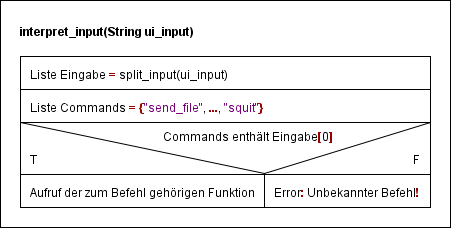
\includegraphics[scale=0.75]{templ}\\
\caption{Grundlegende Struktur der Interpreterfunktion}
\label{intp}
\end{figure}



%\begin{lstlisting}[caption = {Interpreter Funktion}]
%function interpret_input(ui_input)
%    local content = split_input(ui_input)
%    local commands = {
%        ["send_file"]=0,
%        ["send_comm"]=0,
%        ["get"]=0,
%        ["open"]=0,
%        ["shutdown"]=0}
%    if commands[content[1]]~=NIL then
%        local result = _G[content[1]](content)
%        print(result)
%    else
%        local name = debug.getinfo(1, "n").name..": "
%        local subject = string.format("%q",content[1])
%        print("ERROR: "..name..subject.." - unbekannter Befehl!")
%    end
%end
%\end{lstlisting}\hfill\\
Die Variable $content$ (in der Abbildung \ref{intp} $Eingabe$ genannt) ist eine Liste der eingegebenen Wörter. Sie wird durch die Funktion $split\_input$ erstellt, welche die rohe eingegebene Zeichenkette an den Leerzeichen teilt, und demnach wortweise abspeichert. In der Liste $commands$ wird der Befehlssatz gespeichert. 
Hierbei wird dem Namen von jedem verfügbaren Befehl ein Wert zugeordnet. Es spielt keine Rolle, welcher Wert es ist, wichtig ist, dass die Variablen initialisiert sind und nicht keinen zugeordneten Wert haben. 
In der folgenden $If-Else$-Struktur wird überprüft, ob der eingegebene Befehl ein Teil des Befehlssatzes ist, sprich, ob in der Liste $commands$ ein Wert für den gewünschten Befehl vorliegt. 
Ist dies nicht der Fall, gibt die Funktion einen Fehler der Form \glqq$ERROR: interpret\_content: EINGABE - unbekannter Befehl!$\grqq\ aus, und es wird keine Übertragung eingeleitet. 
Wenn die eingegebene Anweisung Teil des Befehlssatzes ist, so wird die entsprechende Funktion mit den übergebenen Parametern aufgerufen, und das Ergebnis in der Variable $result$ gespeichert. 
Der Aufruf geschieht durch die Lua-Interne Funktion $.G[STRING](ARGUMENTS)$, welche eine Zeichenkette als Input fordert, und eine Funktion dieses Namens mit den gewünschten Argumenten $ARGUMENTS$ aufruft.\\\\

\begin{figure}[h!]
\label{fkts}
\caption{Strukturelle Darstellung der grundlegenden Funktionsstruktur}
\end{figure}
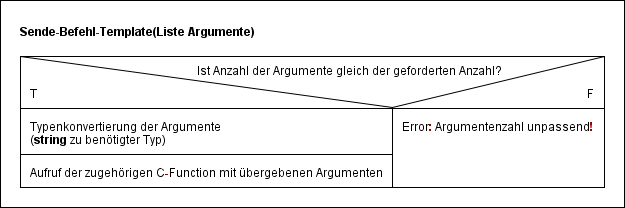
\includegraphics[scale=0.75]{inp}\\

Die gewählte Form der Implementierung, dass der Befehlssatz in einer Liste, bestehend aus den Namen der zugehörigen Funktionen, gespeichert ist, ermöglicht eine unkomplizierte Erweiterung der grundlegenden Befehle durch neue Funktionalität, welche möglicherweise spezifischere Ansprüche an das Protokoll fordert. 
Beispiel hierfür ist die Implementierung von Streaming, die einen ständigen Erhalt der Netzwerkverbindung zwischen den zwei Rechnern benötigen würde. \\
Die eigentlichen Funktionen sind alle nach einem ähnlichen Schema aufgebaut. 
Es gibt zwei verschachtelte $If-Else$-Bedingungen, die erfüllt werden müssen um die eigentliche Übertragung auszulösen. 
In der ersten wird überprüft, ob die gewünschte Übertragung autorisiert ist. 
Dies ist der Fall, wenn auf dem Computer, an den die Übertragung gerichtet ist, der Verbindung zugestimmt wurde. 
Die zweite Bedingung prüft, ob die Anzahl der gegebenen Argumente mit der Anzahl an geforderten Argumenten übereinstimmt. 
Schlägt eine der Bedingungen fehl, so wird der Vorgang abgebrochen und eine Fehlermeldung entsprechend der oben dargestellten Form ausgegeben. 
Sind beide Forderungen erfüllt, werden die Argumente, welche als Zeichenkette eingegeben wurden, in die notwendigen Datentypen konvertiert und die zu den Funktionen zugehörigen Anbindungen an das Netzwerkprotokoll initialisiert.  \\\hfill\\


%\begin{lstlisting}[caption = {Beispielhafte Sende Funktion}]
%function send_NAME(args)
%local name = debug.getinfo(1, "n").name
%    if get_length(args)==INTEGER then
%        local ARG1 = args[2]
%        ...
%        local ARGN = args[N+1]
%        if authenticate(ip) then
%            local blank = "c_sendNAME(ARG1, ..., ARGN))"
%        else
%        	local type = " - Uebertragung wurde abgelehnt"
%            print("ERROR: "..name..type)
%        end
%    else
%    	local type = " - Argumentenzahl unpassend"
%        print("ERROR: "..name..type)
%    end
%end
%\end{lstlisting}
%\newpage

%\end{document}
